% =====================================================================================
% ToonSense — Methodology section
% Required packages: graphicx, booktabs, amsmath, amssymb, multirow, (hyperref)
% Figures: figures/methodology_flow.pdf   |   Bibliography: references.bib
% Numbers in this section come from results/<dataset>/ and results/RESULTS.md (CMBan: 133-meme labelled subset,
% coarse labels; BanglaAbuseMeme and MemoSen: released labels).
% =====================================================================================

\section{Methodology}
\label{sec:method}

\subsection{Overview}
\label{sec:method:overview}

Figure~\ref{fig:flow} summarises ToonSense. The design separates the two modalities. Text is recovered from the
meme image with optical character recognition (OCR) and encoded by a frozen multilingual language model. The image
is encoded by a frozen vision encoder. A lightweight fusion head is trained on the two embeddings for each semantic
task. On top of this pipeline, linguistic and visual perturbations are injected \emph{before} the encoders, so the
same trained classifiers are evaluated on clean and perturbed versions of the same memes. The resulting predictions
feed four analyses: clean evaluation, robustness analysis, explainability, and error analysis. A fifth stage tests
whether the dominant failure can be mitigated by train-time data augmentation. The full protocol is applied to three
Bangla meme datasets.

Following the proposal, all pretrained encoders are kept frozen and their embeddings are pre-computed. This makes the
study computationally feasible and isolates the effect of a perturbation: a perturbation only changes the input to
an encoder, never the classifier that is evaluated.

\begin{figure*}[t]
  \centering
  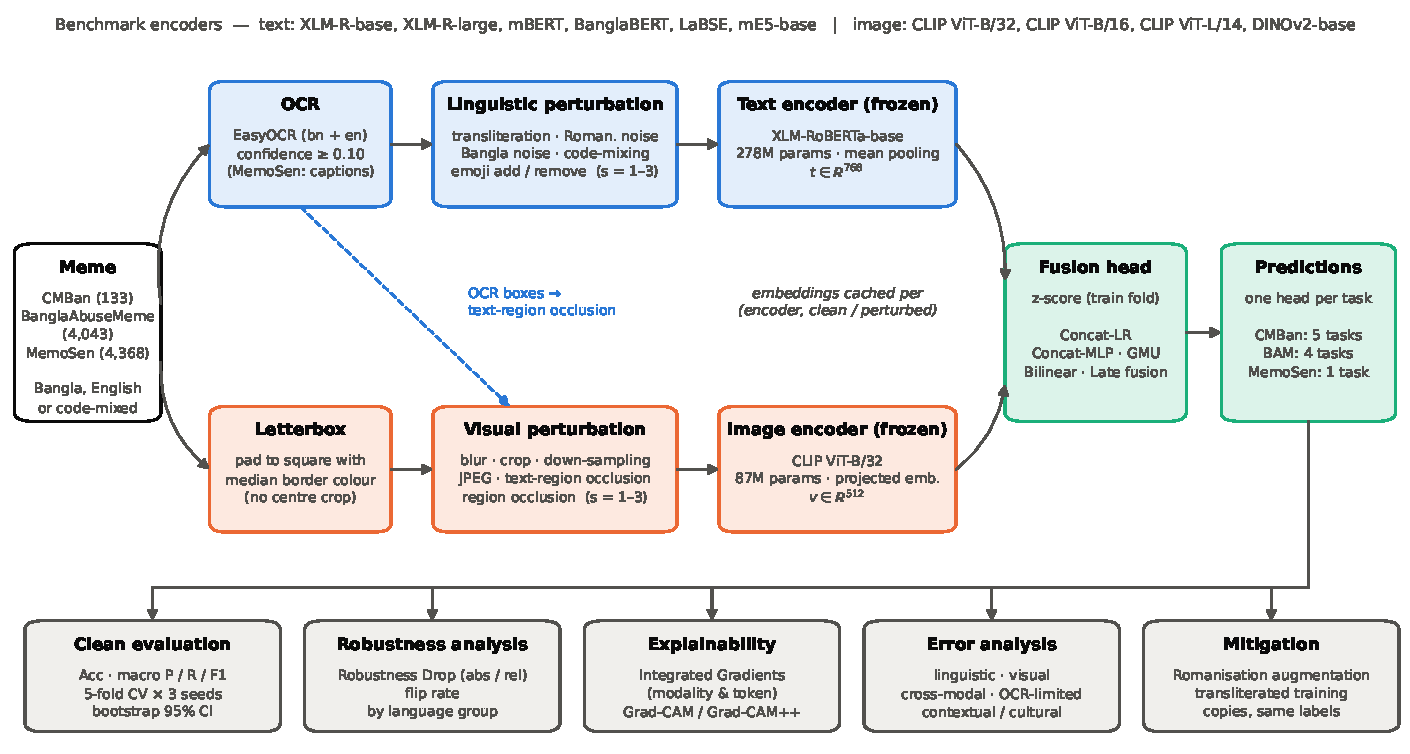
\includegraphics[width=\textwidth]{figures/methodology_flow.pdf}
  \caption{Methodology of ToonSense. Meme text is extracted with OCR (MemoSen: human-written captions) and encoded
  by XLM-RoBERTa-base; the letterboxed image is encoded by CLIP ViT-B/32. Both encoders are frozen. Controlled
  linguistic and visual perturbations (severity $s \in \{1,2,3\}$) are applied before encoding, and a separate fusion
  head is trained for each task of each dataset. OCR bounding boxes are reused to occlude rendered text. Predictions
  on clean and perturbed inputs feed the clean evaluation, robustness, explainability and error analyses, and a
  train-time Romanisation augmentation tests a mitigation. The alternative encoders listed at the top are used in the
  encoder benchmark.}
  \label{fig:flow}
\end{figure*}

% -------------------------------------------------------------------------------------
\subsection{Datasets}
\label{sec:method:data}

Table~\ref{tab:datasets} summarises the three datasets.

\paragraph{CMBan (target dataset).}
CMBan~\cite{cmban2025} contains cartoon-driven memes in Bangla, English and Bangla--English code-mixed language.
Each meme is annotated along five dimensions:
\begin{itemize}
  \item \textit{Humour}: Not Funny / Funny / Very Funny.
  \item \textit{Sarcasm}: Not / Little / Very Sarcastic.
  \item \textit{Offensiveness}: Not / Slight / Hateful Offensive.
  \item \textit{Motivation}: Not Motivational / Motivational.
  \item Overall \textit{Sentiment}: five levels from Very Negative to Very Positive.
\end{itemize}
The paper reports 2{,}641 memes, but the public release (GitHub, Hugging Face and Kaggle) provides labels for only
$N=133$; we use these. By language tag, 85 memes are Bangla, 45 code-mixed and 3 English. Several fine-grained
classes are very small (e.g.\ six \textit{Very Positive} memes). We therefore report CMBan at two granularities: the
original \emph{fine} labels, and \emph{coarse} labels that collapse intensity levels (e.g.\ Funny vs.\ Not Funny;
Negative / Neutral / Positive). Coarse labels are the primary CMBan setting. The label distribution is given in
Table~\ref{tab:data_cmban}.

\paragraph{Larger-scale Bangla meme datasets.}
To test whether our findings hold at scale, we repeat the full protocol on two public Bangla meme datasets whose
labels overlap with CMBan's tasks.
\begin{itemize}
  \item \textbf{BanglaAbuseMeme}~\cite{das2023banglaabusememe} has 4{,}043 memes annotated for sentiment
  (3 classes), sarcasm, abuse and vulgarity. Its text is rendered in the image, so it goes through the same OCR
  pipeline as CMBan.
  \item \textbf{MemoSen}~\cite{hossain2022memosen} has 4{,}368 memes with three-way sentiment and
  \emph{human-written} captions. We use the captions as the text modality, which removes OCR noise. OCR is still
  run on MemoSen to locate text regions for occlusion.
\end{itemize}
Sentiment and sarcasm correspond directly to CMBan tasks, and abuse/vulgarity are close to CMBan's offensiveness.
Neither dataset carries language tags, so we assign each meme a script group from its text: \emph{Bangla} if at
least 85\% of its letters are Bangla script, \emph{Latin-script} if at most 15\% are (English or Romanised Bangla,
which script alone cannot separate), and \emph{code-mixed} otherwise.

\begin{table*}[t]
\centering
\small
\caption{Datasets. ``Text'' is the source of the text modality; CMBan classes are given at the fine level (coarse
level in parentheses).}
\label{tab:datasets}
\begin{tabular}{lrll}
\toprule
Dataset & $N$ & Tasks (classes) & Text \\
\midrule
CMBan (released subset) & 133     & humour 3 (2), sarcasm 3 (2), offensive 3 (2), motivational 2 (2), sentiment 5 (3) & OCR \\
BanglaAbuseMeme         & 4{,}043 & sentiment (3), sarcasm (2), abuse (2), vulgarity (2)                             & OCR \\
MemoSen                 & 4{,}368 & sentiment (3)                                                                    & human \\
\bottomrule
\end{tabular}
\end{table*}

\begin{table}[t]
\centering
\small
\caption{CMBan: Label distribution of the labelled CMBan subset (N=133).}
\label{tab:data_cmban}
\begin{tabular}{lcc}
\toprule
Task & Class & n (\%) \\
\midrule
humour & Not Funny & 57 (42.9) \\
humour & Funny & 59 (44.4) \\
humour & Very Funny & 17 (12.8) \\
sarcasm & Not Sarcastic & 57 (42.9) \\
sarcasm & Little Sarcastic & 40 (30.1) \\
sarcasm & Very Sarcastic & 36 (27.1) \\
offensive & Not Offensive & 99 (74.4) \\
offensive & Slight Offensive & 20 (15.0) \\
offensive & Hateful Offensive & 14 (10.5) \\
motivational & Not Motivational & 83 (62.4) \\
motivational & Motivational & 50 (37.6) \\
sentiment & Very Negative & 11 (8.3) \\
sentiment & Negative & 25 (18.8) \\
sentiment & Neutral & 61 (45.9) \\
sentiment & Positive & 30 (22.6) \\
sentiment & Very Positive & 6 (4.5) \\
\bottomrule
\end{tabular}
\end{table}


% -------------------------------------------------------------------------------------
\subsection{Pre-processing}
\label{sec:method:prep}

\paragraph{Text extraction.}
CMBan and BanglaAbuseMeme memes carry their text \emph{inside} the image, so the text modality is obtained with
EasyOCR~\cite{easyocr} using its Bangla and English recognition models. Images whose longest side exceeds
1{,}280\,px are down-scaled before recognition. Detected fragments with confidence below $0.10$ are discarded, and
the remaining fragments are ordered top-to-bottom in line bands and left-to-right within a band.
\begin{itemize}
  \item On CMBan, OCR returns non-empty text for every meme, with a mean fragment confidence of $0.58$ and a mean
  length of 24.8 words.
  \item On BanglaAbuseMeme, the mean confidence is $0.54$ and the mean length 15.5 words.
  \item On MemoSen, the human-written captions (mean length 14.8 words) are used as text. OCR is still run, to obtain
  text boxes and OCR confidences.
\end{itemize}
The bounding box of every fragment is stored and later reused for text-region occlusion
(Section~\ref{sec:method:pert}).

\paragraph{Image normalisation.}
CLIP-style processors resize the shorter side and then centre-crop to a square. For tall multi-panel comics, which
are common in CMBan, this removes the first and last panels. We therefore \emph{letterbox} each image to a square,
padding with its median border colour, before the encoder's standard $224\times224$ preprocessing. The encoder thus
sees the complete meme.

% -------------------------------------------------------------------------------------
\subsection{Encoders}
\label{sec:method:enc}

\paragraph{Primary configuration.}
The primary model pairs \textbf{XLM-RoBERTa-base} (XLM-R)~\cite{conneau2020xlmr} as the text encoder with
\textbf{CLIP ViT-B/32}~\cite{radford2021clip} as the image encoder. For XLM-R, a text is tokenised (at most 256
tokens) and mean-pooled over the final hidden states, giving $\mathbf{t}\in\mathbb{R}^{768}$. For CLIP, we use the
projected image embedding of the vision tower, $\mathbf{v}\in\mathbb{R}^{512}$. Both encoders are frozen.

\paragraph{Benchmark encoders.}
To situate this choice, we benchmark six text and four image encoders (Table~\ref{tab:encoders}).
\begin{itemize}
  \item Text, multilingual: XLM-R-large~\cite{conneau2020xlmr} and mBERT~\cite{devlin2019bert}.
  \item Text, Bangla-specific: BanglaBERT~\cite{bhattacharjee2022banglabert}.
  \item Text, sentence-embedding models: LaBSE~\cite{feng2022labse} and multilingual-E5-base~\cite{wang2024me5}.
  \item Image, language-supervised: CLIP ViT-B/16 and ViT-L/14~\cite{radford2021clip}.
  \item Image, self-supervised (no language supervision): DINOv2-base~\cite{oquab2024dinov2}.
\end{itemize}

\begin{table}[t]
\centering
\small
\caption{Frozen encoders. Parameter counts are for the encoder actually used (for CLIP, the vision tower only).
$^\star$ marks the primary configuration.}
\label{tab:encoders}
\begin{adjustbox}{max width=\columnwidth}
\begin{tabular}{llrrl}
\toprule
Modality & Encoder & Params & Dim. & Pooling \\
\midrule
\multirow{6}{*}{Text}
 & XLM-R-base$^\star$ & 278M & 768  & mean \\
 & XLM-R-large        & 560M & 1024 & mean \\
 & mBERT (cased)      & 178M & 768  & mean \\
 & BanglaBERT         & 110M & 768  & mean \\
 & LaBSE              & 471M & 768  & pooler, $\ell_2$ \\
 & mE5-base           & 278M & 768  & mean, $\ell_2$ \\
\midrule
\multirow{4}{*}{Image}
 & CLIP ViT-B/32$^\star$ & 87M  & 512  & projection \\
 & CLIP ViT-B/16         & 86M  & 512  & projection \\
 & CLIP ViT-L/14         & 303M & 768  & projection \\
 & DINOv2-base           & 87M  & 1536 & [CLS; mean patch] \\
\bottomrule
\end{tabular}
\end{adjustbox}
\end{table}

% -------------------------------------------------------------------------------------
\subsection{Fusion and Classification Heads}
\label{sec:method:heads}

Embeddings are z-score standardised with statistics from the training fold only. A separate head is trained for each
task. Let $\mathbf{t}$ and $\mathbf{v}$ be the standardised text and image embeddings, $H=256$ the hidden size, and
$C$ the number of classes.

\paragraph{Unimodal heads.}
(i) An $\ell_2$-regularised logistic regression (LR). (ii) A two-layer MLP:
$\mathrm{Dropout}\!\to\!\mathrm{Linear}(d,H)\!\to\!\mathrm{GELU}\!\to\!\mathrm{Dropout}\!\to\!\mathrm{Linear}(H,C)$.

\paragraph{Early fusion.}
The LR or MLP above applied to the concatenation $[\mathbf{t};\mathbf{v}]$ (\emph{Concat-LR}, \emph{Concat-MLP}).

\paragraph{Gated Multimodal Unit (GMU).}
Following~\cite{arevalo2017gmu}, a learned gate decides, per hidden unit, how much each modality contributes:
\begin{equation}
\begin{aligned}
\mathbf{h}_t&=\tanh(W_t\mathbf{t}),\quad \mathbf{h}_v=\tanh(W_v\mathbf{v}),\quad \mathbf{z}=\sigma\!\left(W_z[\mathbf{t};\mathbf{v}]\right),\\
\mathbf{h}&=\mathbf{z}\odot\mathbf{h}_t+(1-\mathbf{z})\odot\mathbf{h}_v ,
\end{aligned}
\end{equation}
followed by a linear classifier on $\mathbf{h}$. The mean gate value is logged as a measure of reliance on text.

\paragraph{Bilinear interaction.}
Both modalities are projected to a shared space, $\mathbf{a}=\tanh(P_t\mathbf{t})$ and
$\mathbf{b}=\tanh(P_v\mathbf{v})$, and an MLP classifies
$[\mathbf{a};\,\mathbf{b};\,\mathbf{a}\odot\mathbf{b};\,|\mathbf{a}-\mathbf{b}|]$. This captures multiplicative
cross-modal interactions.

\paragraph{Late fusion.}
The class probabilities of the text-MLP and image-MLP are averaged:
$\hat{p}=\tfrac12\big(p_{\text{text}}+p_{\text{image}}\big)$.

\paragraph{Baselines.}
A majority-class predictor, and a character $n$-gram ($n=2$--$5$) TF-IDF + LR classifier on the OCR text. The latter
is script-agnostic and therefore a strong lexical baseline for code-mixed input.

\paragraph{Training.}
Neural heads are trained full-batch with AdamW (learning rate $10^{-3}$, weight decay $10^{-2}$), dropout $0.3$ and
class-weighted cross-entropy, for at most 300 epochs. Early stopping (patience 30) is based on the loss on an inner
validation split, and the best checkpoint is restored. For the LR heads, the inverse regularisation strength
$C\in\{0.01,0.1,1\}$ is selected on the same validation split, with balanced class weights.

% -------------------------------------------------------------------------------------
\subsection{Rationale for XLM-R + CLIP ViT-B/32}
\label{sec:method:why}

We adopt XLM-R-base + CLIP ViT-B/32 as the primary configuration for the reasons below. We stress that the choice
rests on the \emph{accuracy--efficiency trade-off} and on suitability for the data, \emph{not} on this pair
achieving the highest clean score in our benchmark.

\begin{enumerate}
  \item \textbf{Coverage of Bangla and code-mixing.} XLM-R is pretrained on CommonCrawl text in 100 languages,
  Bengali included~\cite{conneau2020xlmr}. Its SentencePiece vocabulary represents Bangla script, English and
  Romanised Bangla within a single model. This matters for CMBan, where 34\% of the labelled memes are code-mixed.
  A Bangla-only model such as BanglaBERT is not designed for English or Romanised tokens.

  \item \textbf{Language-supervised visual features.} CLIP is trained contrastively on image--text
  pairs~\cite{radford2021clip}. Its embedding therefore encodes the high-level semantics (scenes, characters,
  expressions) that meme interpretation depends on, rather than low-level appearance alone.

  \item \textbf{Competitive accuracy.} Among the 51 fusion configurations of the benchmark, the best primary head is
  1.7 (CMBan), 1.9 (BanglaAbuseMeme) and 2.6 (MemoSen) macro-F1 points behind the top configuration
  (Table~\ref{tab:cross_bench}). On CMBan the gap is not significant after Holm correction. Almost all of the gap is
  due to the image encoder: every top configuration uses CLIP ViT-L/14, which is 2.7--2.8 points better than
  ViT-B/32 as a unimodal model on all three datasets. The text encoder matters much less. With CLIP ViT-B/32 as the
  image encoder, XLM-R-base is the best text partner on CMBan (49.6\% vs.\ $\leq$48.3\%; best head per task) and
  within 0.2 points of the best on BanglaAbuseMeme and MemoSen.

  \item \textbf{Efficiency.} CLIP ViT-B/32 is the smallest image encoder considered (87M parameters). It encodes
  the 133 memes in about 15\,s on a CPU, compared with about 150\,s for ViT-L/14 (303M). XLM-R-large doubles the
  parameter count of XLM-R-base (560M vs.\ 278M) yet improves the text-only task-averaged macro-F1 by only 0.1--2.4
  points across the three datasets. The robustness protocol re-encodes 36 perturbed variants of the data, so encoder
  cost multiplies. The smaller pair keeps the CMBan study runnable on a CPU and the full study on the larger
  datasets within a single free GPU session (about 4--6\,h on a Tesla T4 per dataset).

  \item \textbf{Comparability.} XLM-R and CLIP are among the most widely used encoders in multimodal meme research,
  which makes our robustness findings comparable with prior work. The full benchmark
  (Section~\ref{sec:results:benchmark}) reports every alternative, so readers can judge the trade-off themselves.
\end{enumerate}

% -------------------------------------------------------------------------------------
\subsection{Controlled Perturbations}
\label{sec:method:pert}

We design six linguistic and six visual perturbation families, each at three severities
(Table~\ref{tab:perturbations}), mirroring how memes are altered as they circulate on social media. Every
perturbation is deterministic given the meme identifier, family and severity (a CRC32-seeded generator), so all
models see identical perturbed inputs. For linguistic perturbations, we record the token-level edit rate
(one minus the \texttt{difflib} similarity ratio over whitespace tokens) to report how much of each text actually
changed.

\paragraph{Linguistic.}
\begin{itemize}
  \item \emph{Transliteration} uses a rule-based Bangla$\to$Romanised-Bangla converter written for this study. It
  follows colloquial social-media conventions rather than a formal scheme: inherent-vowel insertion, schwa deletion
  word-finally and in VC\_CV contexts, \textit{ya-}/\textit{ba-phala}, and nukta forms.
  \item \emph{Romanised spelling noise} first romanises the text fully, then applies common Banglish spelling
  variants (e.g.\ \textit{sh}$\leftrightarrow$\textit{s}, \textit{bh}$\to$\textit{v}, \textit{i}$\to$\textit{ee},
  vowel dropping, character repetition, adjacent swaps).
  \item \emph{Bangla spelling noise} substitutes orthographically confusable characters (short/long vowel signs,
  the three sibilants, dental/retroflex nasals, etc.) or drops a vowel sign.
  \item \emph{Code-mixing} switches words between Bangla and English using a bilingual lexicon of about 200
  frequent meme words, with Bangla suffix stripping.
  \item \emph{Emoji insertion} inserts emojis from a mixed-sentiment pool.
  \item \emph{Emoji removal} strips emojis, then emoticons, then all symbols.
\end{itemize}

\paragraph{Visual.}
\begin{itemize}
  \item Blur strength is defined at the encoder's $224$-px scale, so it is independent of image resolution.
  \item \emph{Text-region occlusion} fills OCR text boxes with their median colour, removing the rendered text
  while adding minimal artefacts.
  \item \emph{Region occlusion} greys out cells of a $12\times12$ grid, restricted to cells that overlap OCR text
  by less than 20\%. It removes pictorial evidence while leaving the text intact.
\end{itemize}

\begin{table}[t]
\centering
\small
\caption{Perturbation families and severities ($s=1/2/3$).}
\label{tab:perturbations}
\begin{adjustbox}{max width=\columnwidth}
\begin{tabular}{lll}
\toprule
 & Family & Parameter at $s=1/2/3$ \\
\midrule
\multirow{6}{*}{\rotatebox{90}{Linguistic}}
 & Transliteration          & 33 / 66 / 100\% of Bangla words romanised \\
 & Romanised spelling noise & 15 / 30 / 50\% of words varied (after full romanisation) \\
 & Bangla spelling noise    & 10 / 20 / 35\% of Bangla words misspelt \\
 & Code-mixing              & switch probability 0.33 / 0.66 / 1.0 \\
 & Emoji insertion          & 1 / 3 / 6 emojis \\
 & Emoji removal            & emojis / + emoticons / + all symbols \\
\midrule
\multirow{6}{*}{\rotatebox{90}{Visual}}
 & Gaussian blur     & $\sigma$ = 1 / 2 / 4 (224-px scale) \\
 & Random crop       & 85 / 70 / 55\% of area kept \\
 & Down-sampling     & longest side 160 / 96 / 48\,px, then up-sampled \\
 & JPEG compression  & quality 30 / 15 / 5 \\
 & Text-region occl. & 33 / 66 / 100\% of OCR boxes filled \\
 & Region occlusion  & 10 / 25 / 40\% of non-text area greyed \\
\bottomrule
\end{tabular}
\end{adjustbox}
\end{table}

In the main (\emph{decoupled}) setting, a linguistic perturbation changes only the text input and a visual
perturbation changes only the image input. This attributes each effect to a single modality. A \emph{coupled}
variant, in which the text of a visually perturbed meme is re-extracted by OCR, is supported by the framework and
models deployment conditions.

% -------------------------------------------------------------------------------------
\subsection{Evaluation Protocol}
\label{sec:method:eval}

\paragraph{Cross-validation.}
On the labelled CMBan subset, a single held-out test split would contain about 27 memes and give unstable estimates.
We therefore use stratified 5-fold cross-validation, repeated with three random seeds, and apply the same protocol
to BanglaAbuseMeme and MemoSen so that all results are directly comparable.
\begin{itemize}
  \item In each fold, 80\% of the memes are used for training and 20\% for testing.
  \item A stratified 15\% of the training portion is held out as the validation split for early stopping and
  hyperparameter selection, so test folds are never used for model selection.
  \item Each meme receives exactly one out-of-fold (OOF) prediction per seed, and all metrics are computed on the
  full set of OOF predictions.
\end{itemize}

\paragraph{Metrics.}
We report accuracy and macro-averaged precision, recall and F1, as mean $\pm$ standard deviation over seeds. Macro-F1
is the primary metric because of class imbalance:
\begin{equation}
\text{Macro-F1}=\frac{1}{C}\sum_{c=1}^{C}\frac{2\,P_c R_c}{P_c+R_c}.
\end{equation}
We compute 95\% confidence intervals by bootstrap resampling (1{,}000 resamples) of the seed-ensembled predictions.
The best fusion model is compared with the best text-only and best image-only models using a paired bootstrap test,
with Holm correction across the tasks of each dataset~\cite{holm1979}. For CMBan, each task is reported at its
primary (coarse) level; the fine level is reported in the appendix.

\paragraph{Robustness.}
Each fold's model is trained once on clean data and then applied to the clean and perturbed versions of its own test
fold. For a model $f$, data $\mathcal{D}$ and perturbation $\pi_s$ at severity $s$, the \emph{Robustness Drop} is
\begin{equation}
\begin{aligned}
\mathrm{RD}_{\text{abs}}&=\mathrm{F1}(f;\mathcal{D})-\mathrm{F1}\big(f;\pi_s(\mathcal{D})\big),\\
\mathrm{RD}_{\text{rel}}&=100\cdot\frac{\mathrm{RD}_{\text{abs}}}{\mathrm{F1}(f;\mathcal{D})}.
\end{aligned}
\end{equation}
Because macro-F1 is noisy on small test sets, we also report the label-free \emph{flip rate}: the fraction of memes
whose prediction changes under the perturbation,
$\mathrm{FR}=\frac{1}{N}\sum_{i}\mathbf{1}\big[f(x_i)\neq f(\pi_s(x_i))\big]$.
All robustness measures are additionally broken down by language group: Bangla, code-mixed and (on BanglaAbuseMeme
and MemoSen) Latin-script memes. Robustness is evaluated for the primary encoder pair and all of its heads, over
$12$ families $\times$ $3$ severities $=36$ perturbed copies of every test fold.

% -------------------------------------------------------------------------------------
\subsection{Mitigation: Romanisation Augmentation}
\label{sec:method:aug}

Romanisation turns out to be the most damaging perturbation (Section~\ref{sec:results:rob}). We therefore test
whether it can be mitigated by train-time data augmentation, without collecting new labels. Let $\mathcal{T}$ be the
training portion of a fold and $\mathcal{V}\subset\mathcal{T}$ its inner validation split. The augmented training
set adds a copy of every non-validation training meme in which only the text is replaced by its perturbed version,
\begin{equation}
\mathcal{T}_{\text{aug}}=\mathcal{T}\;\cup\;\big\{\big(\pi_{s}(t_i),\,\mathbf{v}_i,\,y_i\big)
\;:\; i\in\mathcal{T}\setminus\mathcal{V},\ \pi_s\in\Pi\big\},
\end{equation}
where $\mathbf{v}_i$ is the clean image embedding and $y_i$ the original label. Copies are never made of validation
or test memes, so model selection and evaluation are not contaminated. We compare three settings:
\begin{itemize}
  \item \emph{none}: clean training data, identical to the robustness analysis.
  \item \emph{+translit.}: $\Pi=\{$transliteration, $s=2\}$. Romanised spelling noise is \emph{not} seen during
  training, so performance under it measures generalisation to an unseen Romanisation style.
  \item \emph{+translit.\ + noise}: $\Pi=\{$transliteration, $s=2$; Romanised spelling noise, $s=2\}$, an upper
  bound in which the test-time noise style is also seen during training.
\end{itemize}
All other components (primary encoder pair, text-only and fusion heads, folds and seeds) are those of the
robustness analysis, so differences are attributable to the augmentation alone. Each setting is evaluated on the
clean test folds and on all linguistic perturbations at all severities. The Robustness Drop is computed relative to
the clean macro-F1 of the same setting, so that any change in clean accuracy is reported separately.

% -------------------------------------------------------------------------------------
\subsection{Explainability}
\label{sec:method:xai}

\paragraph{Modality reliance.}
We apply Integrated Gradients (IG)~\cite{sundararajan2017ig} to the input $\mathbf{x}=[\mathbf{t};\mathbf{v}]$ of the
fusion head, using the training mean as baseline $\mathbf{x}'$ and $m=32$ midpoint Riemann steps:
\begin{equation}
\mathrm{IG}_j(\mathbf{x})=(x_j-x'_j)\int_{0}^{1}
\frac{\partial F_{\hat{y}}\big(\mathbf{x}'+\alpha(\mathbf{x}-\mathbf{x}')\big)}{\partial x_j}\,d\alpha ,
\end{equation}
where $F_{\hat{y}}$ is the logit of the predicted class. The \emph{text share} of a decision is
$\|\mathrm{IG}_{\mathbf{t}}\|_1/(\|\mathrm{IG}_{\mathbf{t}}\|_1+\|\mathrm{IG}_{\mathbf{v}}\|_1)$. It is computed
for every meme on clean and perturbed inputs to measure how perturbations shift reliance between modalities.

\paragraph{Token attribution.}
For memes whose correct prediction flips under a linguistic perturbation, IG is propagated through XLM-R to the input
token embeddings, using a pad-token baseline that keeps special tokens fixed. Sub-word attributions are summed into
words, and the clean and perturbed texts are compared.

\paragraph{Visual attribution.}
We apply Grad-CAM~\cite{selvaraju2017gradcam} and Grad-CAM++~\cite{chattopadhay2018gradcampp} to CLIP ViT-B/32 by
treating the patch tokens as a spatial feature map. The hook is placed at the \emph{input} of the last transformer
block: at its output, only the class token reaches the projection, so patch gradients would vanish. With
activations $A\in\mathbb{R}^{P\times D}$ and target logit $y^{c}$,
\begin{equation}
w_k=\frac{1}{P}\sum_{p}\frac{\partial y^{c}}{\partial A_{p,k}},\qquad
L^{c}_{p}=\mathrm{ReLU}\Big(\sum_k w_k A_{p,k}\Big).
\end{equation}
From the map we derive two quantities:
\begin{itemize}
  \item The \emph{text-attention ratio}: the share of CAM mass inside OCR text boxes divided by the boxes' share of
  the image area. A value above 1 means the model over-attends to rendered text.
  \item \emph{CAM stability}: the Pearson correlation between clean and perturbed maps, computed for the spatially
  aligned perturbations (blur, JPEG, down-sampling and both occlusions) at severity 2.
\end{itemize}
IG modality shares are computed for every meme. Grad-CAM requires a backward pass through CLIP per meme and
perturbation, so on the two larger datasets it is computed on a stratified subsample of at most 300 memes per task.

% -------------------------------------------------------------------------------------
\subsection{Error Analysis}
\label{sec:method:errors}

Errors of the primary fusion model (the best \emph{learned} XLM-R + CLIP-B/32 fusion head per task) are attributed
to a source by comparing its seed-ensembled out-of-fold predictions with those of the text-MLP and image-MLP trained
on the same folds. Late fusion is excluded here: it averages the two unimodal models, so for binary tasks it cannot
be wrong when both are right, and the cross-modal category would be empty by construction. The categories are:
\begin{itemize}
  \item \emph{linguistic}: the text model is wrong and the image model right.
  \item \emph{visual}: the image model is wrong and the text model right.
  \item \emph{cross-modal}: both unimodal models are right but fusion is wrong.
  \item \emph{OCR-limited}: all three models are wrong and the OCR text is empty or has confidence below 0.5.
  \item \emph{contextual/cultural}: all three models are wrong although usable text is available.
\end{itemize}
The contextual/cultural category is treated as a set of \emph{candidates}, which annotators verify for cultural
references.

Robustness failures are categorised analogously. A meme is \emph{linguistic-}, \emph{visual-} or
\emph{cross-modal-fragile} if its correct clean prediction becomes wrong at severity $\geq2$ under a linguistic
perturbation, a visual perturbation, or both. It is \emph{stable} if it is classified correctly on clean data and
under every perturbation.

% -------------------------------------------------------------------------------------
\subsection{Implementation and Compute}
\label{sec:method:impl}

The pipeline is implemented in Python with PyTorch, Hugging Face Transformers, scikit-learn and EasyOCR. It
consists of separate scripts for OCR, feature extraction, benchmark, robustness, explainability, error analysis,
augmentation, reporting and cloud packaging. Every step caches its outputs.
Embeddings are computed once per encoder and input variant (clean or perturbed) and reused by all heads, folds and
seeds.

\begin{itemize}
  \item \textbf{CMBan} runs end-to-end on a laptop CPU.
  \item \textbf{BanglaAbuseMeme and MemoSen} were run on a Kaggle Tesla T4 GPU session, about 4--6\,h per dataset.
  The largest costs are the 51-configuration benchmark (1.5--2.7\,h) and the re-encoding of the 36 perturbed
  copies (0.7--1.1\,h).
  \item \textbf{The augmentation experiment} needs no encoder pass: it reuses the cached embeddings and trains only
  the heads, on CPU.
\end{itemize}

All random choices are seeded. Perturbations are deterministic per meme, family and severity, and folds and head
initialisations are determined by the seed. A unit-test suite checks the transliterator, the determinism and
monotonic severity of every perturbation, the metrics, the isolation of modalities in the cross-validation engine,
and the absence of validation or test leakage in the augmentation.
